% arara: pdflatex
% arara: latexmk: { clean: partial }
\documentclass[tikz]{standalone}
\usepackage{tikz}
\usepackage{../../../../glossary}


\begin{document}
        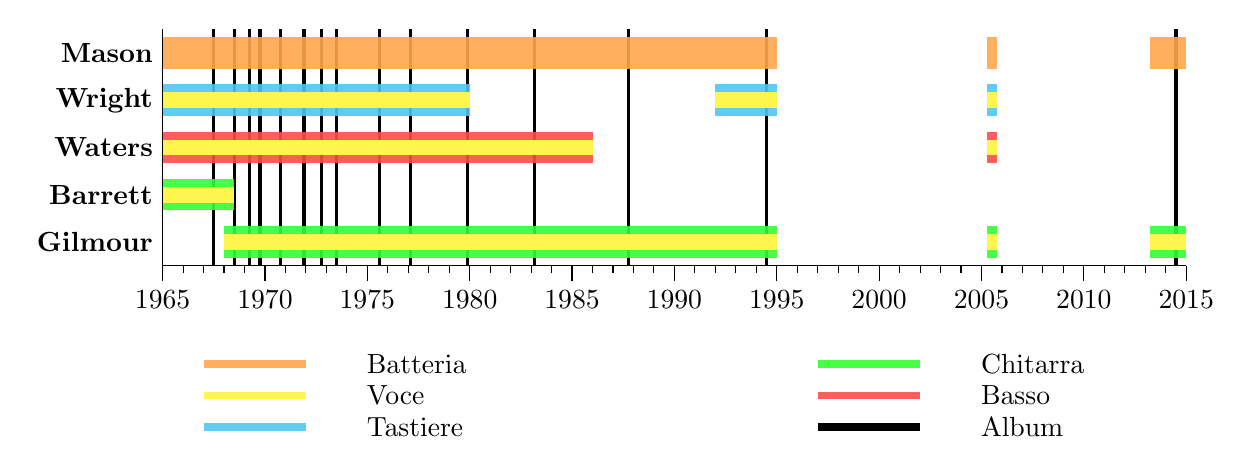
\begin{tikzpicture}[xscale=13] % Adjust xscale for A4 width
        % Draw the timeline
        \draw[-] (0, 0) -- (1, 0) node[right] {};

        \draw[-] (0, 0) -- (0, 3);

        % Define year offsets
        \def\ySixtyFive{0.000}
        \def\ySeventy{0.100}
        \def\ySeventyFive{0.200}
        \def\yEighty{0.300}
        \def\yEightyFive{0.400}
        \def\yNinety{0.500}
        \def\yNinetyFive{0.600}
        \def\yTwoThousand{0.700}
        \def\yTwoThousandFive{0.800}
        \def\yTwoThousandTen{0.900}
        \def\yTwoThousandFifteen{1.000}

        \def\memberHeight{0.4}
        \def\memberOffset{0.2}

        % Add ticks and labels
        \foreach \x/\label in {
            \ySixtyFive/1965,
            \ySeventy/1970,
            \ySeventyFive/1975,
            \yEighty/1980,
            \yEightyFive/1985,
            \yNinety/1990,
            \yNinetyFive/1995,
            \yTwoThousand/2000,
            \yTwoThousandFive/2005,
            \yTwoThousandTen/2010,
            \yTwoThousandFifteen/2015
        } {
            \draw (\x, 0) -- (\x, -0.2); % Ticks
            \node[below] at (\x, -0.2) {\label}; % Labels
        }

        \foreach \decade in {
            \ySixtyFive,
            \ySeventy,
            \ySeventyFive,
            \yEighty,
            \yEightyFive,
            \yNinety,
            \yNinetyFive,
            \yTwoThousand,
            \yTwoThousandFive,
            \yTwoThousandTen
        } {
            \foreach \offset in {0.020, 0.040, 0.060, 0.080} {
                \draw (\decade + \offset, 0) -- (\decade + \offset, -0.1); % Ticks
                \node[below] at (\decade + \offset, -0.2) {}; % Empty labels
            }
        }

        % Vertical bars at significant dates
        \draw[black, very thick] (\ySixtyFive + 0.05, 3) -- (\ySixtyFive + 0.05, 0); 
        \draw[black, very thick] (\ySixtyFive + 0.07, 3) -- (\ySixtyFive + 0.07, 0); 
        \draw[black, very thick] (\ySixtyFive + 0.085, 3) -- (\ySixtyFive + 0.085, 0); 
        \draw[black, very thick] (\ySixtyFive + 0.095, 3) -- (\ySixtyFive + 0.095, 0); 
        \draw[black, very thick] (\ySeventy + 0.015, 3) -- (\ySeventy + 0.015, 0); 
        \draw[black, very thick] (\ySeventy + 0.038, 3) -- (\ySeventy + 0.038, 0); 
        \draw[black, very thick] (\ySeventy + 0.055, 3) -- (\ySeventy + 0.055, 0); 
        \draw[black, very thick] (\ySeventy + 0.070, 3) -- (\ySeventy + 0.070, 0); 
        \draw[black, very thick] (\ySeventyFive + 0.012, 3) -- (\ySeventyFive + 0.012, 0); 
        \draw[black, very thick] (\ySeventyFive + 0.042, 3) -- (\ySeventyFive + 0.042, 0); 
        \draw[black, very thick] (\ySeventyFive + 0.098, 3) -- (\ySeventyFive + 0.098, 0); 
        \draw[black, very thick] (\yEighty + 0.063, 3) -- (\yEighty + 0.063, 0); 
        \draw[black, very thick] (\yEightyFive + 0.055, 3) -- (\yEightyFive + 0.055, 0); 
        \draw[black, very thick] (\yNinety + 0.09, 3) -- (\yNinety + 0.09, 0); 
        \draw[black, very thick] (\yTwoThousandTen + 0.09, 3) -- (\yTwoThousandTen + 0.09, 0); 

        % Member timelines
        % Syd Barrett
        \fill[green!80, opacity=0.9] (0, 1.1) rectangle (\ySixtyFive + 0.07, 0.7);

        \fill[yellow!70, opacity=1] (0, 1) rectangle (\ySixtyFive + 0.07, 0.8);

        \node[left] at (0, 0.9) {\textbf{Barrett}};

        % David Gilmour
        \fill[green!80, opacity=0.9] (\ySixtyFive + 0.06, 0.5) rectangle (\yNinetyFive, 0.1);
        \fill[green!80, opacity=0.9] (\yTwoThousandFive + 0.005, 0.5) rectangle (\yTwoThousandFive + 0.015, 0.1);
        \fill[green!80, opacity=0.9] (\yTwoThousandTen + 0.065, 0.5) rectangle (1, 0.1);

        \fill[yellow!70, opacity=1] (\ySixtyFive + 0.06, 0.4) rectangle (\yNinetyFive, 0.2);
        \fill[yellow!70, opacity=1] (\yTwoThousandFive + 0.005, 0.4) rectangle (\yTwoThousandFive + 0.015, 0.2);
        \fill[yellow!70, opacity=1] (\yTwoThousandTen + 0.065, 0.4) rectangle (1, 0.2);

        \node[left] at (0, 0.3) {\textbf{Gilmour}};

        % Roger Waters  
        \fill[red!70, opacity=0.9] (0, 1.7) rectangle (\yEightyFive + 0.02, 1.3);
        \fill[red!70, opacity=0.9] (\yTwoThousandFive + 0.005, 1.7) rectangle (\yTwoThousandFive + 0.015, 1.3);

        \fill[yellow!70, opacity=1] (0, 1.6) rectangle (\yEightyFive + 0.02, 1.4);
        \fill[yellow!70, opacity=1] (\yTwoThousandFive + 0.005, 1.6) rectangle (\yTwoThousandFive + 0.015, 1.4);

        \node[left] at (0, 1.5) {\textbf{Waters}};

        % Richard Wright
        \fill[cyan!70, opacity=0.9] (0, 2.3) rectangle (\yEighty, 1.9);
        \fill[cyan!70, opacity=0.9] (\yTwoThousandFive + 0.005, 2.3) rectangle (\yTwoThousandFive + 0.015, 1.9);
        \fill[cyan!70, opacity=0.9] (\yNinety + 0.04, 2.3) rectangle (\yNinetyFive, 1.9);

        \fill[yellow!70, opacity=1] (0, 2.2) rectangle (\yEighty, 2);
        \fill[yellow!70, opacity=1] (\yTwoThousandFive + 0.005, 2.2) rectangle (\yTwoThousandFive + 0.015, 2);
        \fill[yellow!70, opacity=1] (\yNinety + 0.04, 2.2) rectangle (\yNinetyFive, 2);

        \node[left] at (0, 2.1) {\textbf{Wright}};

        % Nick Mason
        \fill[orange!70, opacity=0.9] (0, 2.9) rectangle (\yNinetyFive, 2.5);
        \fill[orange!70, opacity=0.9] (\yTwoThousandFive + 0.005, 2.9) rectangle (\yTwoThousandFive + 0.015, 2.5);
        \fill[orange!70, opacity=0.9] (\yTwoThousandTen + 0.065, 2.9) rectangle (1, 2.5);

        \node[left] at (0, 2.7) {\textbf{Mason}};

        % Legend (below visualization)
        \begin{scope}[yshift=-1cm, xshift=-0.36cm]
            % First column
            \fill[orange!70, opacity=0.9] (0.4, -0.2) rectangle (0.5, -0.3);
            \node[right] at (0.55, -0.25) {Batteria};
            \fill[yellow!70, opacity=1] (0.4, -0.6) rectangle (0.5, -0.7);
            \node[right] at (0.55, -0.65) {Voce};
            \fill[cyan!70, opacity=0.9] (0.4, -1) rectangle (0.5, -1.1);
            \node[right] at (0.55, -1.05) {Tastiere};
            % Second column
            \fill[green!80, opacity=0.9] (1.0, -0.2) rectangle (1.1, -0.3);
            \node[right] at (1.15, -0.25) {Chitarra};
            \fill[red!70, opacity=0.9] (1.0, -0.6) rectangle (1.1, -0.7);
            \node[right] at (1.15, -0.65) {Basso};
            \fill[black!, opacity=1] (1.0, -1) rectangle (1.1, -1.1);
            \node[right] at (1.15, -1.05) {Album};
        \end{scope}
    \end{tikzpicture}
\end{document}